\subsection{Misuratori software e modelli di stima}

Le limitazioni intrinseche dei misuratori hardware, quali la scarsa granularità
temporale, i costi elevati di implementazione su larga scala e l’impossibilità di
attribuire direttamente il consumo energetico a singole entità logiche in sistemi
multi-tenant, hanno favorito l’emergere dei misuratori software.
Questi strumenti non si basano su sensori fisici dedicati per ogni applicazione,
ma utilizzano modelli di stima che correlano l’attività del software con il consumo
energetico complessivo del sistema.
Il principio fondamentale consiste nell’impiegare metriche di utilizzo delle
risorse hardware — come cicli di clock della CPU, istruzioni eseguite, accessi alla
cache e operazioni di input/output — come base per stimare l’energia
assorbita dalle singole entità di esecuzione.
Questo approccio consente di ottenere una visibilità energetica più granulare
rispetto alle sole misure hardware, risultando particolarmente adatto a contesti
moderni quali il cloud computing, le architetture a microservizi e i sistemi
containerizzati.

Uno dei framework più rappresentativi in questo ambito è PowerAPI, una libreria modulare progettata per il monitoraggio del consumo energetico a livello di processo attraverso componenti indipendenti e meccanismi di raccolta dati asincroni e scalabili
\cite{fieni:hal-02470128}. L’architettura di PowerAPI è progettata per separare nettamente la fase di raccolta
delle metriche da quella di stima energetica, favorendo l’estendibilità e la
portabilità del sistema. Il pilastro tecnologico di PowerAPI è rappresentato dall’\textbf{HWPC Sensor}
(\textit{Hardware Performance Counter Sensor}), un componente specializzato nel
campionamento ad alta frequenza dei contatori di prestazione hardware
\cite{powerapi-hwpc}.
Il sensore si interfaccia direttamente con il sottosistema \texttt{perf\_event} del
kernel Linux, permettendo di raccogliere metriche dettagliate sull’attività della
CPU associate a specifici \textit{Control Groups} (cgroups)
\footnote{Il sottosistema \texttt{perf\_event} del kernel Linux fornisce
un’interfaccia unificata per il monitoraggio di eventi hardware e software a basso
livello, come cicli di clock della CPU, istruzioni eseguite e cache miss.
Attraverso la chiamata di sistema \texttt{perf\_event\_open()}, consente di associare
le misurazioni a processi, thread o \textit{cgroups}, esponendo i dati tramite
\textit{file descriptor} e buffer ad anello con overhead contenuto.
\texttt{perf\_event} costituisce inoltre la base del tool \texttt{perf}, ampiamente
utilizzato per la profilazione delle prestazioni nei sistemi Linux.} In parallelo, l’HWPC Sensor interroga i \textit{Model Specific Registers} (MSR)
tramite l’interfaccia \textit{Running Average Power Limit} (RAPL), ottenendo misure
cumulative del consumo energetico dei principali domini della CPU
\cite{rapl-evaluation}.

La Figura~\ref{fig:powerapi-architecture} mostra una rappresentazione concettuale
dell’architettura di PowerAPI.
Le metriche di utilizzo delle risorse e le informazioni energetiche fornite dai
sensori hardware vengono elaborate dal modello di stima \textbf{SmartWatts}, adottato
da PowerAPI per attribuire il consumo energetico ai singoli processi.

\begin{figure}[t]
    \centering
    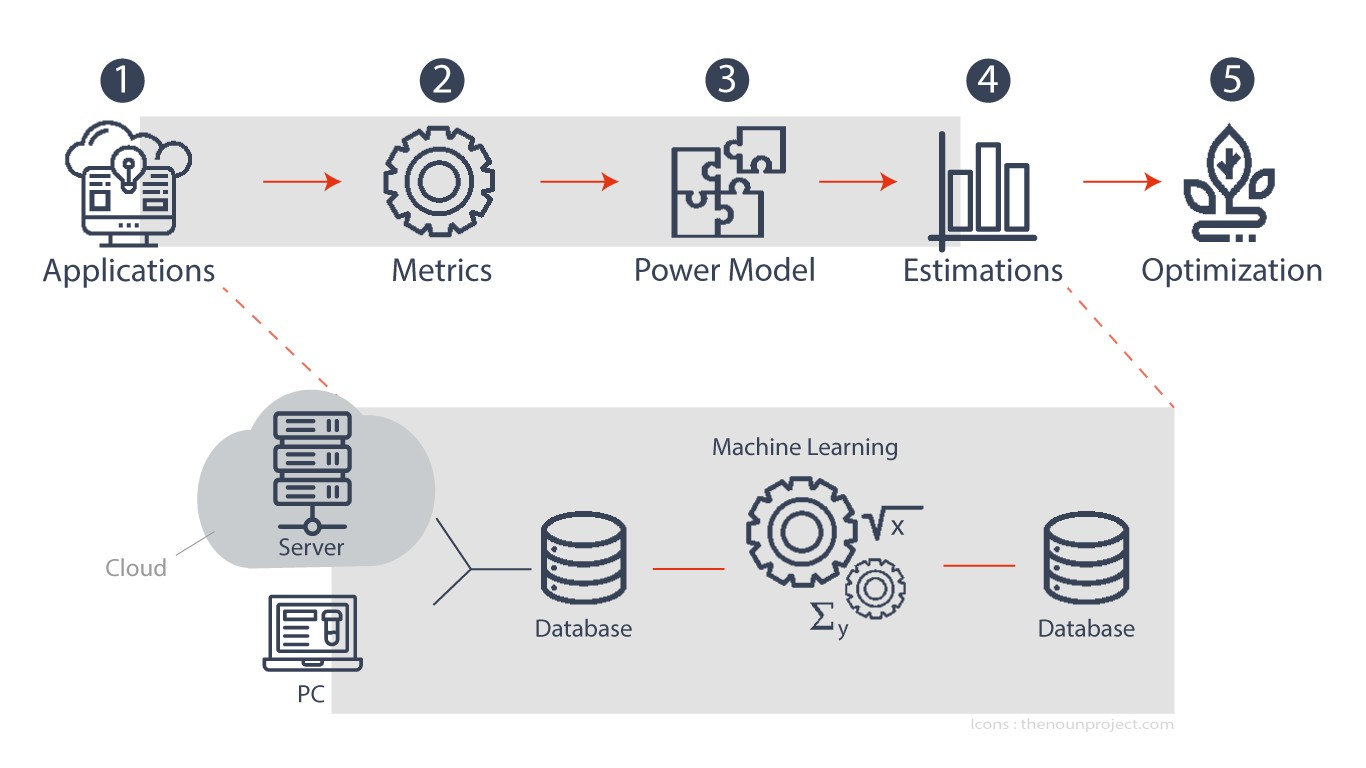
\includegraphics[width=0.9\textwidth]{figures/PowerApi.jpg}
    \caption{Architettura concettuale di PowerAPI. I contatori di prestazione hardware
    e le misure energetiche aggregate (RAPL) vengono combinati dal modello SmartWatts
    per stimare il consumo energetico dei singoli processi.}
    \label{fig:powerapi-architecture}
\end{figure}

SmartWatts utilizza tecniche di regressione lineare per scomporre il consumo
energetico globale in una componente statica e una dinamica, consentendo
un’attribuzione più accurata rispetto a modelli puramente statici
\cite{powerapi-smartwatts}.
Tale approccio richiede una fase di auto-calibrazione \textit{online} e l’accesso
diretto all’hardware sottostante.

Tali requisiti rendono PowerAPI particolarmente adatto a scenari \textit{bare-metal},
ma ne limitano l’applicabilità in ambienti virtualizzati e cloud pubblici, dove
l’accesso ai registri hardware della CPU e ai performance counter è spesso inibito
dagli hypervisor per motivi di sicurezza e isolamento.
In questi contesti emerge la necessità di strumenti di monitoraggio energetico
progettati nativamente per ambienti orchestrati.

Un approccio rappresentativo in questa direzione è \textbf{Kepler}
(\textit{Kubernetes-based Efficient Power Level Exporter}), un progetto
\textit{cloud-native} orientato al monitoraggio energetico di container e Pod in
cluster Kubernetes \cite{kepler-medium,kepler-redhat2}.
A differenza di PowerAPI, Kepler non richiede accesso diretto ai registri hardware
della CPU, ma sfrutta la tecnologia \textit{eBPF} (\textit{Extended Berkeley Packet
Filter}) per raccogliere metriche a livello kernel in modo non intrusivo e con
overhead computazionale ridotto.

La Figura~\ref{fig:kepler-architecture} mostra l’architettura complessiva di Kepler.
Il sistema utilizza un \textit{eBPF Program Generator} per generare dinamicamente
programmi eBPF che vengono agganciati ai \textit{tracepoint} del kernel e ai
performance counter della CPU.
Questi programmi intercettano eventi di schedulazione e statistiche di esecuzione,
consentendo di associare l’attività computazionale ai singoli container in modo
fine-grained.

Le informazioni raccolte tramite eBPF vengono arricchite dal \textit{Pod Lister},
che interroga le API di Kubernetes per mappare gli identificativi dei container ai
rispettivi Pod e raccoglie statistiche aggiuntive dai \textit{control groups}.
Parallelamente, il componente \textit{Energy Stats Reader} acquisisce informazioni
energetiche aggregate dal nodo, utilizzando diverse fonti a seconda della
disponibilità dell’hardware sottostante, tra cui RAPL, sensori hardware esterni,
interfacce GPU (NVML) e modelli basati su benchmark standardizzati.

Quando le misure hardware dirette non risultano accessibili, scenario tipico delle
macchine virtuali nei cloud pubblici, Kepler ricorre a modelli di stima basati su
\textit{Machine Learning}, denominati \textit{Estimators}.
Tali modelli, addestrati offline su differenti architetture hardware e carichi di
lavoro, ricevono in input le metriche raccolte a livello kernel e producono una
stima della potenza assorbita dai container, che viene successivamente integrata nel
tempo per ottenere una stima energetica complessiva.

Le metriche prodotte da Kepler vengono infine esposte tramite un \textit{Prometheus
Exporter}, rendendo il consumo energetico direttamente interrogabile attraverso i
meccanismi di \textit{scraping} standard e facilmente integrabile con strumenti di
visualizzazione.
Questa integrazione nativa con l’ecosistema di osservabilità cloud consente di
affiancare le metriche energetiche a quelle di performance, abilitando analisi
congiunte e politiche di gestione consapevoli dal punto di vista energetico.
\begin{figure}[t]
    \centering
    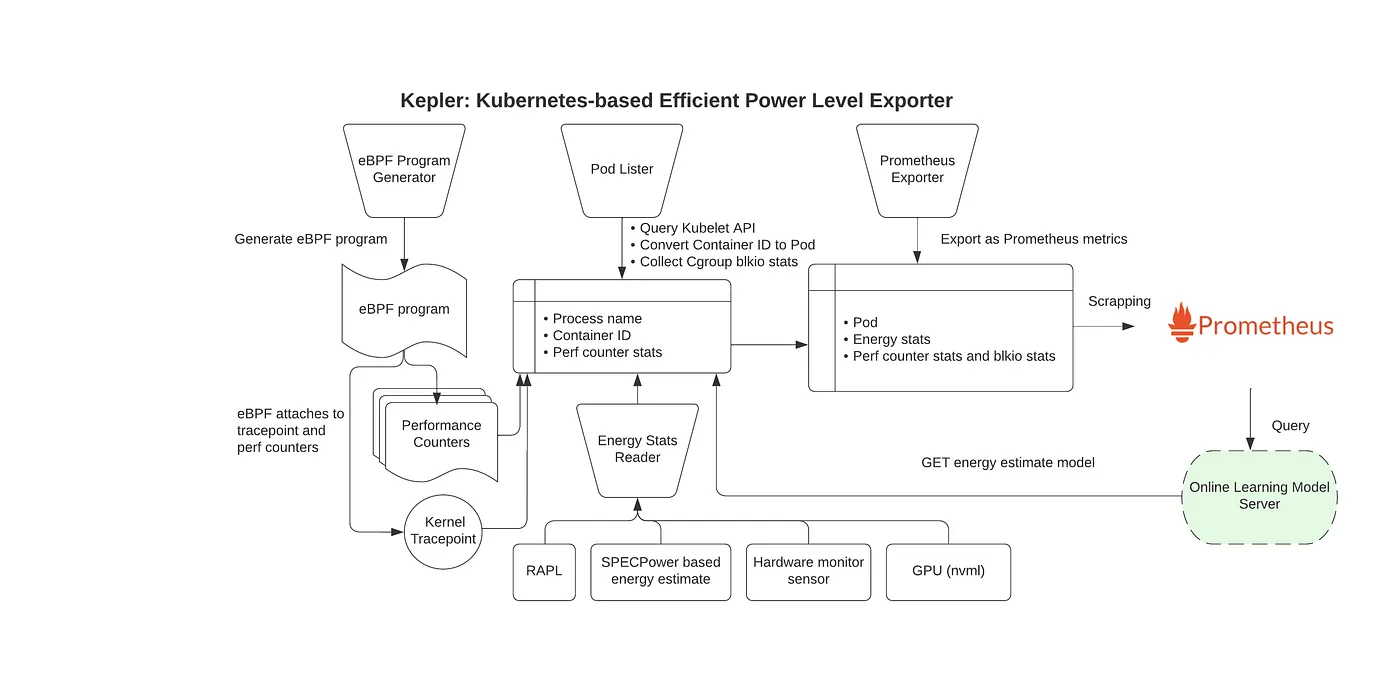
\includegraphics[width=0.75\textwidth]{figures/Kepler.png}
    \caption{Architettura di Kepler.}
    \label{fig:kepler-architecture}
\end{figure}
